\chapter{Monte Carlo corrections}
Monte Carlo plays important role in cross-section measurement. It is constantly undergoing correction to data, in order to obtain a required precision. Part of this corrections have been described in a chapter \ref{chap:MC}. Unfortunatelly,  not everything can be taken into account during simulation itself. This leads to a differences between data and monte carlo, that needs to be accounted for. There are two possible methods to correct monte carlo without regenerating it. First on is to apply event weight, so what each mc event can contribute to non 1 entries in a histogram.This is called reweighting. Second one is to smear MC. It is using random number to alter reconstructed 4-vectors. 
This chapter describes all additional corrections, what have been applied on MC in this analysis. All of this correction are introducing additional systematic error, that will be discussed in the chapter \ref{sec:}

\section{Lepton efficiency corrections}

Lepton detection efficiency at \atlas detector can be divided into three components:
\begin{itemize}
\item The reconstruction efficiency $\epsilon_{rec}$ is a probability to reconstruct lepton as a lepton of this flavor.
\item The identification efficiency $\epsilon_{id \mid rec}$ is the probability that a reconstructed lepton survives  identification requirements. 
\item The trigger efficiency $\epsilon_{trig \mid rec,id}$ is the probability, that lepton satisfy trigger requirements. 
\end{itemize}
The full efficiency for a single lepton can be written as:
\begin{equation}
\epsilon_{total}=\epsilon_{rec} \times \epsilon_{id \mid rec} \times \epsilon_{trig \mid rec,id}
\end{equation}
All of this efficiencies are measured using Tag and Probe method in $Z\to ll$ decays. This is allowing to insure, that all of the reconstructed lepton candidates are coming from an actual leptons. One of the leptons from Z boson, called "probe", is initially selected with all of the cuts, minus one under study. Second one, called "probe" satisfies more tighter selection with additional cut, such as, for example, trigger matching.

Reconstruction efficiency is assosiated with algorithm used to perform reconstruction. This is causing difference between electrons and muons efficiencies. In electron case it is a probability to reconstruct an elec tron with an electromagnetic calorimeter as an electron.  Muon reconstruction efficiency is given by:
\begin{equation}
\epsilon_{reco,muon} = \epsilon_{reco,muon|ID} \cdot \epsilon_{ID} \approx \epsilon_{reco,muon|ID} \cdot \epsilon_{ID|MS},
\end{equation}
where $\epsilon_{reco,muon|ID}$ is a conditional probability that muon reconstructed in ID is also reconstructed using MS as as a combined muon, and  $\epsilon_{ID}$ is a probability that muon is reconstructed as an ID track. This quantity cannot be measured directly and therefore is replaced by $\epsilon_{ID|MS}$, that can be measured by tag-and-probe method. 
uncertainty in this analysis. 

\begin{figure}[t]
\centering
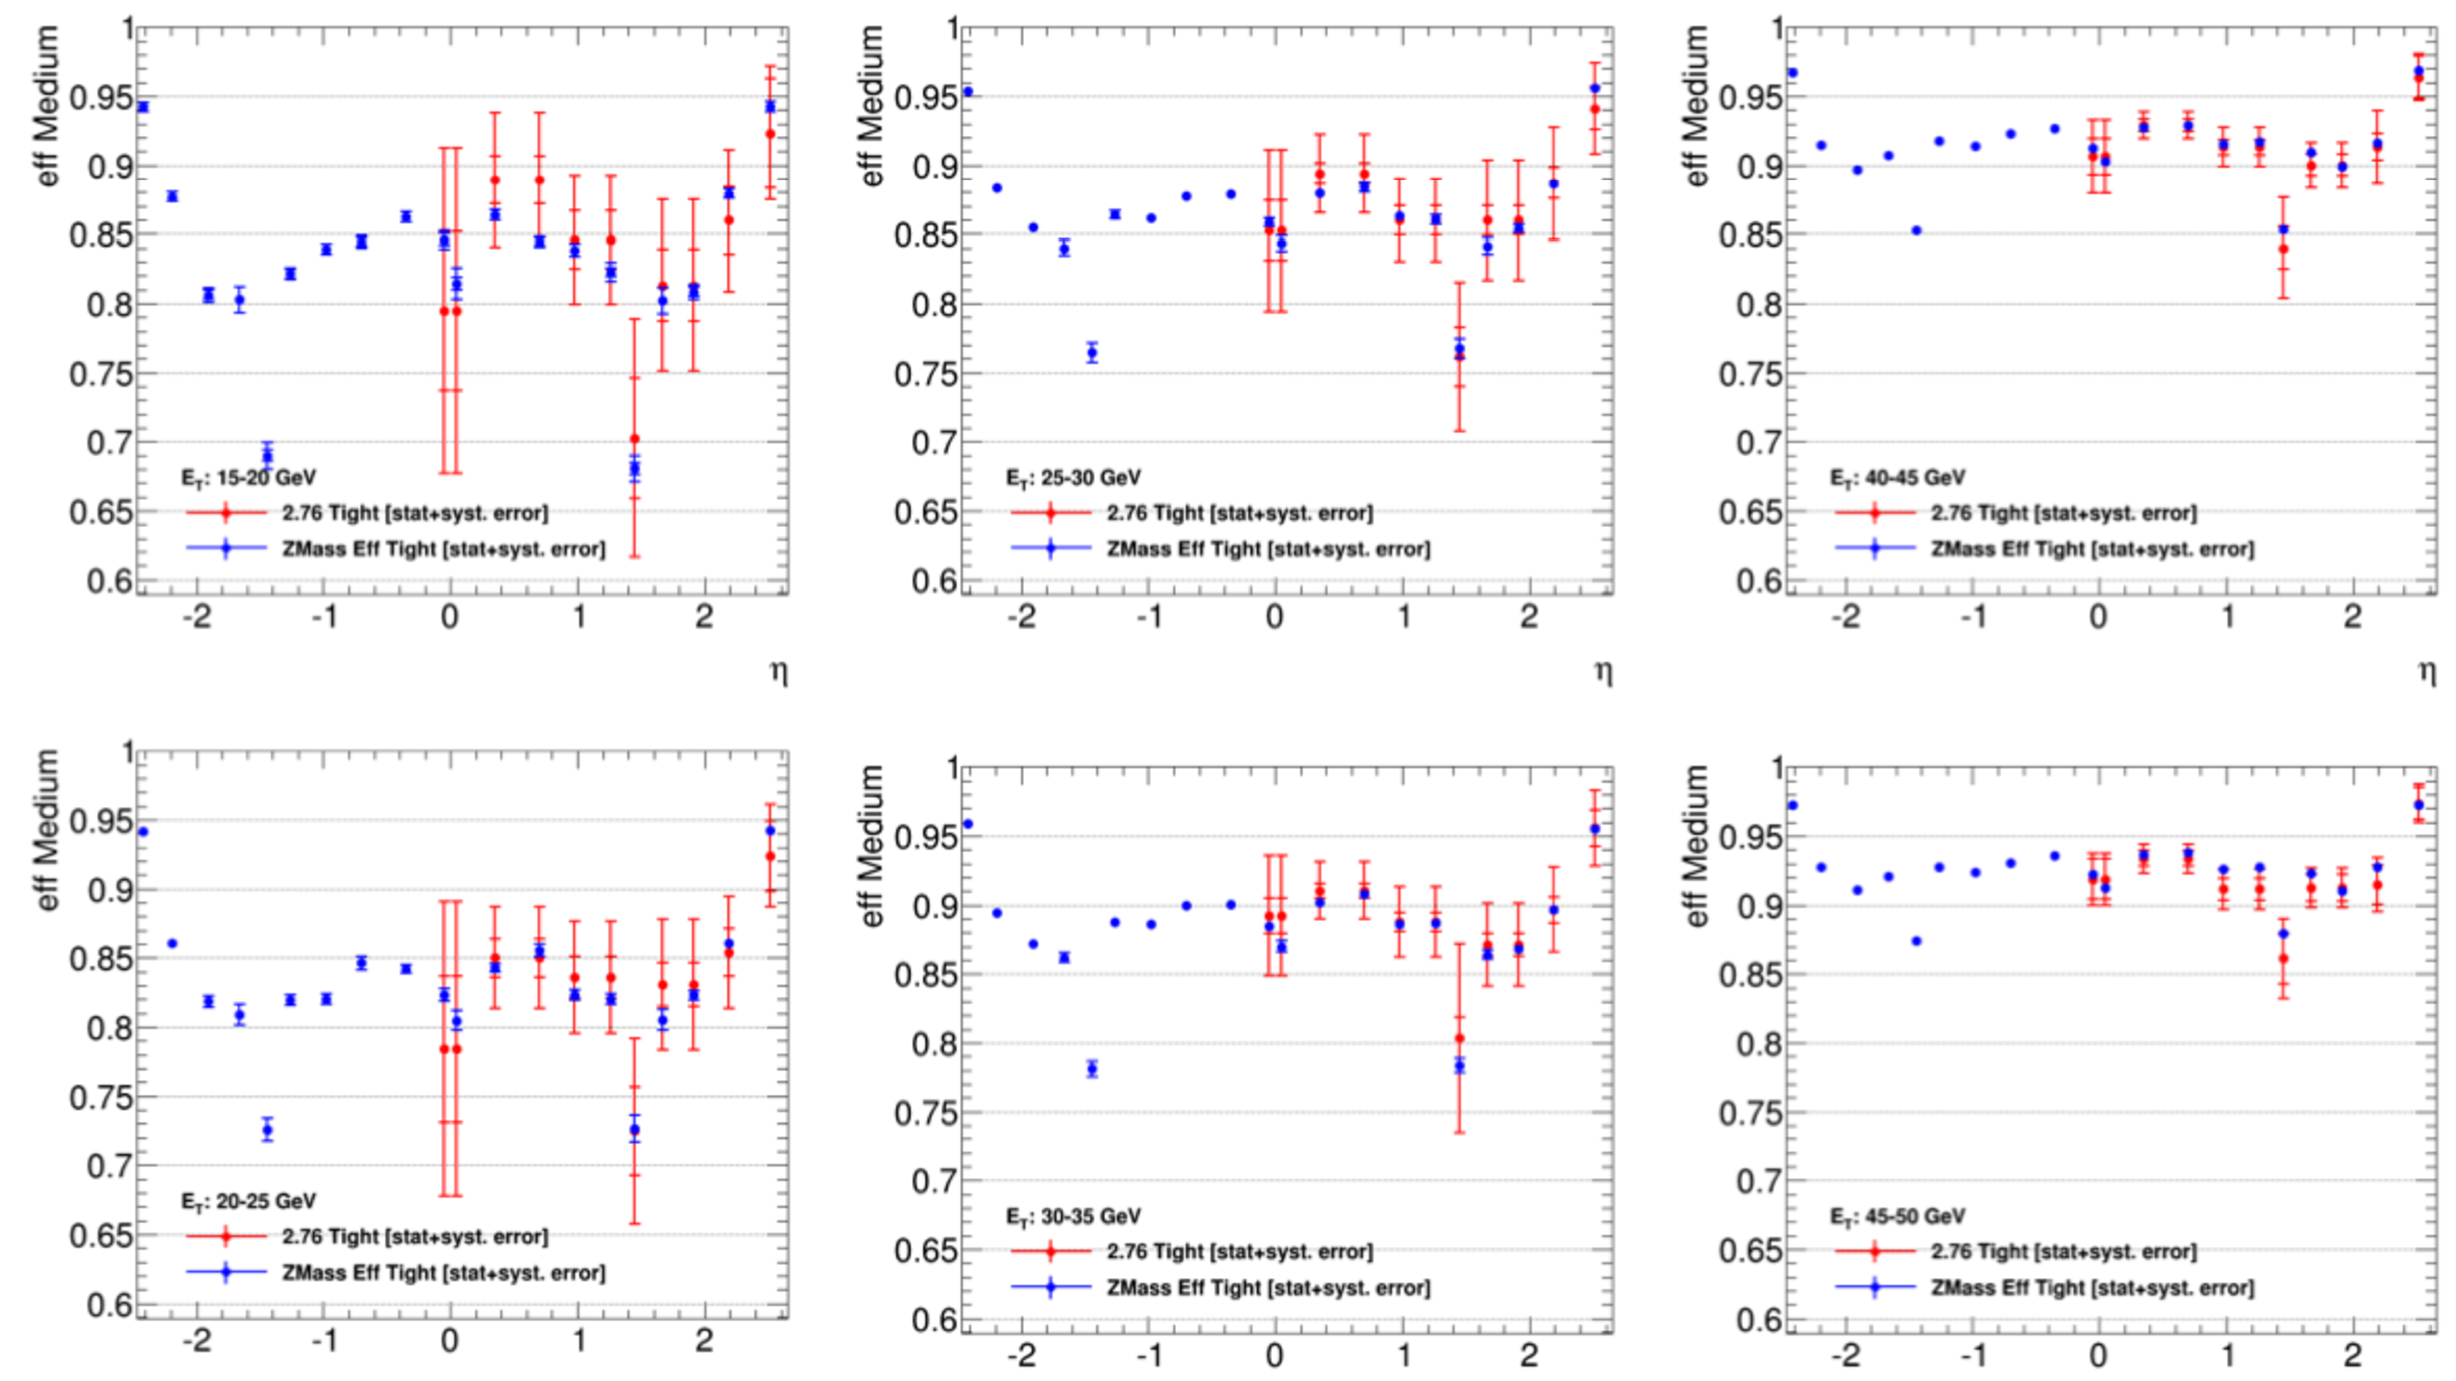
\includegraphics[width=1\textwidth]{MCCorrections/sf.pdf}
\caption{Comparition of electron efficiencies as calculated for 8TeV (blue points) and 2.76TeV (red points) for MC simulation. Efficiencies are shown as a function of pseudorapidity ($\eta$) for different electron $E_T$ bins. Both statistical and systematic uncertainties are shown. }
\label{eff_comp}
\end{figure}
Simulation samples are corrected to match data efficiencies by a scale-factor :
\begin{equation}
SF_{reco,id,trig}=\frac{\epsilon^{data}_{reco,id,trig}}{\epsilon^{MC}_{reco,id,trig}}
\end{equation}

Each of the scale factors calculated in a $p_{t}$ and $\eta$ bins and has an associated statistical and systematical uncertainty component. Statistical component is connected to a size of $Z\to ll$, which is in our case is around 500 event per each lepton flavor. This means that precise calculation of scaling factors based on this data is difficult.

It is possible to use scale factors for 8 TeV 2012 data. The main difference between this data samples are center of mass energy and a pile-up conditions (10 in 2012 and less than 1 in 2013). This effects have been studied on a $Z\to ee$ sample. Fig. \ref{eff_comp} shows that all of the differences in a scale factors are negligible and fully covered by the statistical error. This justifies the usage of 8 TeV scalling factors with increased 

Unfortunatelly, single muon trigger haven't been presented in a 2012 data, so muon trigger scale factor needed to be derived from a 2.76 TeV data. Different configurations is calculated as a single number in order to minimize systematics contribution. 
\section{Electron energy scale and resolution}
Electrons clusters tend to shift in a reconstructed energy compared to a truth energy of initial electron. Correction of this shift is done on a both data and MC as a 3 step process:
\begin{itemize}
\item Electronic calibration, that transfers a raw signal from a readout to a cluster energy deposit.
\item MC based calibration. It corrects effects of energy loss in the material in front of calorimeter and leakage into the hadronic calorimeter. This calibration is applied on both data and MC.
\item Correction of calorimeter cell responce in data. This is allowing to get right responce in non-optimal HV-regions and exclude biases in a calorimeter electronics reconstruction.
\end{itemize}

Energy shift is parameterised, as:
\begin{equation}
E^{data}=E^{MC}(1+\alpha_i),
\end{equation}
where $E^{data}$ and $E^{MC}$ are the energies in data and simulation, respectivelly and $\alpha_i$ is a mean shift in a given bin i in $\eta$. Effect of this miscalibration on a reconstructed mass of Z boson is:
\begin{equation}
m_{i,j}^{data}=m_{i,j}^{MC}(1+\alpha_{i,j}), \quad \alpha_{i,j} \sim \frac{\alpha_i+\alpha_j}{2}
\end{equation}
neglecting second order terms. $m_{i,j}^{data}$ and $m_{i,j}^{MC}$ are reconstructed mass of Z boson in a $i$ and $j$ bins of $\eta$ for data and MC respectivelly. 

There is also a need to correct difference in a electron resolution. It can be desribed by a formula \ref{eq:EMResoultion}. It is assumed, that sampling and noise terms are moddeled well by MC and the main diiference is coming from a constant term. 
So, the electron resoultion correction then can be written as:
\begin{equation}
\frac{\sigma_E}{E}^{Data}_{i}=\frac{\sigma_E}{E}^{MC}_{i} \oplus c_i
\end{equation}
where $c_i$ is $\eta$ dependent relative resolution correction. Similarly to a energy scale correction it is possible to derive resolution correction factor by a comparing $m_{i,j}^{data}$ and $m_{i,j}^{MC}$ distribution. 

Correction values of $\alpha_i$ and $c_i$ are obtained via $\chi^2$ fit on a invariant mass electrons for data and MC. Resulting energy scale is applied on a data, while resolution is corrected for MC. The resulting scale is validated on a $J/\psi \to ee$ and $Z\to ee \gamma$

\section{Muon momentum correction}
Muon momentum resolution is depending on a $\eta$, $\phi$ and $p_T$ of the muon \cite{AtlasExperiment}. There is an impirical formula to describe it inside the detector (ID or MS):
\begin{equation}\label{eq:MuonResolution}
\frac{\sigma_{Det}(p_T)}{p_T}=\frac{r^{Det}_0(\eta, \phi)}{p_T} \oplus r^{Det}_1 (\eta, \phi)  \oplus r^{Det}_2(\eta, \phi) \cdot p_T
\end{equation}

The first term origins from fluctuations of energy loss in transversed material. Second $r^{Det}_1$ is coming from magnetic field inhomogenities and local displacements. Third term $r^{Det}_2$ describes intrinsic resolution effects. 

Similarly to electrons, overall energy scale shift between data and MC parameterised as:
\begin{equation}
p_T^{data}=p_T^{MC}+s_0^{Det}(\eta, \phi)+s_1^{Det}(\eta, \phi) \cdot p_T^{MC},
\end{equation}
where $s_0^{Det}(\eta, \phi)$ is coming from the imperfect knowledge of energy losses for muons passing through detector. 

This leads to a total correction formula:
\begin{equation}
p^{Cor,Det}_T=\frac{p_{T}^{MC,Det}+\sum\limits_{n=0}^1 s_n^{Det}(\eta, \phi)(p_T^{MC,Det})^n}{1+\sum\limits_{m=0}^2 \Delta r_m^{Det}(\eta, \phi)(p_T^{MC,Det})^{m-1} g_m},
\end{equation}
where $g_m$ are normally distributed random variables with mean 0 and width 1. Because small amount of material between interaction point and the ID, $\Delta r^{ID}_0(\eta, \phi)$ and $s_0^{ID}(\eta, \phi)$ are set to 0. Missallignment effect for an MS is corrected on a simulation level by adding a random smearing to an allignment constants. This is allowing to set $\Delta r^{MS}_2(\eta, \phi)$ to 0 during a fit. 

The correction factors are extracted using $Z \to \mu \mu$ candidates events with requirement on a two combined muons. For correction invariant mass distribution $m_{\mu\mu}^ID$ and $m_{\mu\mu}^{MS}$ are considered individually within a specific $\eta - \phi$ region of fit. Combined muon parameters are used to obtain angles $\eta$ $\phi$. 
The correction extraction is performed first for an ID and then for MS with addition of the fit variable:
\begin{equation}
\rho = \frac{p_T^{MS}-p_T^{ID}}{p_T^{ID}},
\end{equation}
which represents $p_T$ imbalance in ID and MS. 

In a second step corrections are propagated to the combined momentum, using a weight average:
\begin{equation}
p_T^{Cor,CB}= f\cdot p_T^{Cor,ID}+(1-f) \cdot p_T^{Cor,MS},
\end{equation}
where weight f is derived from mc. 

\section{Number of vertexes reweighting}
Additional particle interactions can affect many different distributions, including $E_T^{miss}$. Pile-up mismodelling usually accounted by correcting average number of interaction per bunch crossing to match a data. However, \atlas simulation is suited for an ordinary high pile-up runs, so this quantity is not modelled well in a case of 2.76 TeV analysis \ref{ris:Mu.png}. 

Another way is to to apply weight on number of vertexes. This variables have a connection between each other, because each pp interaction produces separate vertex. Fig ~\ref{ris:MC_Nvtx} shows a comparison of number of vertexes before and after reweighting.

This also allows to improve agreement for a $E_T^{miss}$ distribution.

\section{Hadron recoil correction}
Remaining differences between Data and MC in $E_T^{miss}$ are assumed to be due to a $\sum E_T$ mismodelling. This quantity is defined as a scalar sum of all active topo-clusters in the event:
\begin{equation}
\sum E_T = \sum\limits^N_{i=0}|\vec{E_T}|
\end{equation}
This variable is connected with a underlying event activity. 
However, $\sum E_t$ is correlated with a $p_T^W$, what is assumed to be simulated well in a MC. Correction procedure should leave this quantity untouched. In order to do this, correction factors are derived separatelly in a different $p_T^W$ bins and flavours, since $p_T^W$ is reconstructed differently in this channels. Size of this bin is choosen, so what each bin is having around 600 events in a data. Due to a limited statistics, data is a proximated by a polinomial fit. Example of this fit is shown on a Figure \ref{fig:Fit}. After this, weights are obtained by a dividing resulting polinomia by a MC. Weights scale is corrected, so what number of events leaves unchanged in a MC:
\begin{equation}
\int \sum E_T^{MC} = \int \sum E_T^{MC} \cdot w,
\end{equation}
where $w$ are the weights. Total correction factors are shown on a Figure \ref{ris:recoilCor}
The resulting $\sum E_T$ distribution shows good agreement with data, while $p_T^W$ leaves unchanged. This correction is also helping to improve $E_T^miss$ distribution.